\lab{Algorithms}{Multivariate Finite Difference Schemes}{Multivariate Numerical Derivatives}

\objective{Understand how to compute numerically the Jacobian and Hessian of a function.}

The Jacobian is our generalization of the derivative in many dimensions. We can think of it, intuitively, as a tangent plane at a point. The Jacobian is of critical importance in a variety of areas, and we will use it in lab \ref{Ch:Newton} to find zeros of multivariate functions.

Formally, the Jacobian of a function $f:R^n \rightarrow R^m$ is an $m \times n$ matrix. It is defined by the formula:
\[
J_{i,j} = \frac{\partial f_i}{\partial x_j}
\]

We can use finite difference approximations to find partial derivatives in the natural manner:
\[
\frac{\partial f}{\partial x_i} (x) \approx \frac{f(x+h e_i)-f(x)}{h}
\]
where $e_i$ is a unit vector in the $i$th coordinate (the direction $x_i$). Higher order approximations and centered and backwards differences follow by naturally extending this definition.

\begin{problem}
Write a function \li{Jacobian(func,inputs,dim,h,o)} that accepts a function handle, inputs to the function, the function's dimensions, step size $h$, and option o. Based on the option have the function output the Jacobian using either a centered, forward or backward difference.

Test your function on the following $f: \mathbb{R}^2 \to \mathbb{R}^2$:
\[
f(x_1, x_2) = 
\begin{pmatrix}
e^{x_1} sin(x_2) + x_2^3 \\
3x_2 - cos(x_1)
\end{pmatrix}
\] 

Compare your \li{Jacobian} function against the analytically computed derivative on the square $[-1,1]\times[-1,1]$ using ten thousand grid points (100 per side). Which method is faster? What is the maximum error of your function? Make sure to test the different options of your function to maximize performance (including values for $h$, and different types of schemes).
\end{problem}

Given a function from $\mathbb{R}^n \to \mathbb{R}$ sometimes the mixed partial derivatives are useful. In particular the mixed partials will be useful when we study optimization in Volume 2. This information is contained in the Hessian matrix, which is defined by:

\[
H_{i,j} = \frac{\partial^2 f}{\partial x_i \partial x_j}
\]

We can use the following formula to approximate mixed partial derivatives:
\small
\[
\frac{\partial^2 f}{\partial x_i \partial x_j} = \frac{f(x + (e_i + e_j)h) - f(x + (e_i-e_j)h) -f(x + (e_j-e_i)h) + f(x - (e_i + e_j)h)}{4h^2}
\]
\normalsize

\begin{problem}
Write a \ProgrammingLanguage function that numerically calculates the hessian of a given function. Test it on the following function:
\[
f(x,y) = (1-x)^2 + 100(y-x^2)^2
\]
This function is known as the Rosenbrock banana function, or Rosenbrock's valley. It is a common test function for optimization algorithms because it is non-convex and the global minimum is hard to find from certain starting points. A graph is shown in figure \ref{Fig:Rosenbrock}. Compare the output of your function with the analytic solution on the region $[-2,2]\times [0,2]$, using ten thousand points. What is the maximum error of your function?
\end{problem}
\begin{figure}
\begin{center}
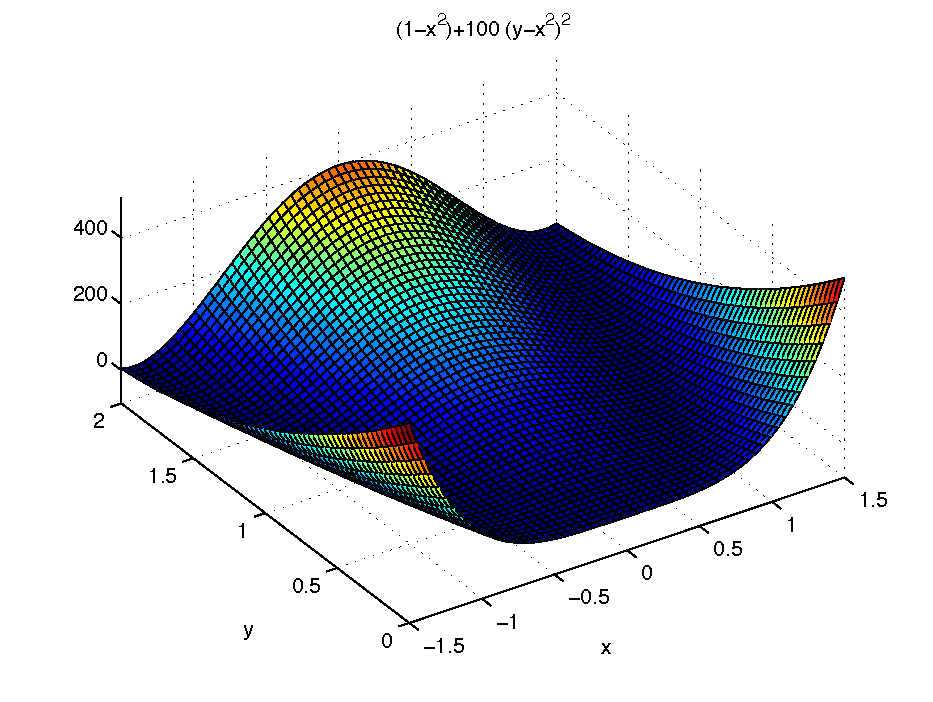
\includegraphics[scale = .8]{./Figures/Rosenbrock}
\caption{The Rosenbrock Banana Function, a common test function in optimization algorithms}
\label{Fig:Rosenbrock}
\end{center}
\end{figure}